\documentclass{../../oss-apphys-exam}

\begin{document}
\genheader

%\genfreetitle{9}{ROTATIONAL MOTION, PART 3}{2}
\begin{center}
  \textbf{
<<<<<<< HEAD
<<<<<<< HEAD
    AP PHYSICS C CLASS 9: ROTATIONAL MOTION, PART 3\\
    2 Questions
=======
    AP PHYSICS C CLASS 9: ROTATIONAL MOTION, PART 3
>>>>>>> 2022-09-fall
=======
    AP PHYSICS C CLASS 9: ROTATIONAL MOTION, PART 3
>>>>>>> ce7a159 (Lots of commits!)
  }
\end{center}
%\genfreedirections

\begin{center}
  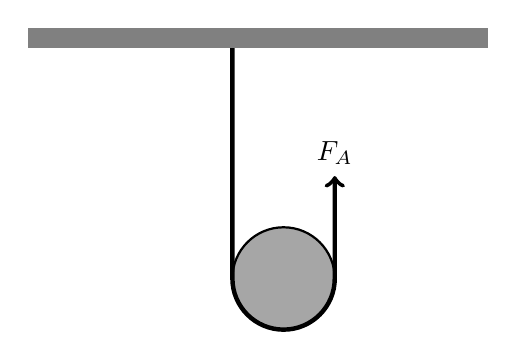
\begin{tikzpicture}[scale=.65]
    \fill[gray!70] circle(1);
    \draw[ultra thick,->](-1,4.5)--(-1,0) arc(180:360:1)
    --(1,2) node[above]{$F_A$};
    \draw[thick](-1,0) arc(180:0:1);
    \fill[gray](-5,4.5) rectangle(4,4.9);
  \end{tikzpicture}
\end{center}

\begin{questions}  
  \question A disk of mass $M =\SI{2.0}{\kilo\gram}$ and radius
  $R=\SI{.10}\metre$ is supported by a rope of negligible mass, as shown
  above. The rope is attached to the ceiling at one end and passes under the
  disk. The other end of the rope is pulled upward with a force $F_A$. The
  rotational inertia of the disk around its center is $MR^2/2$.
  \begin{parts}
    \part Calculate the magnitude of the force $F_A$ necessary to hold the disk
    at rest.
    \vspace{\stretch1}
    
    \uplevel{
      At time $t=0$, the force $F_A$ is increased to 12 N, causing the disk to
      accelerate upward. The rope does not slip on the disk as the disk rotates.
    }

    \part Calculate the linear acceleration of the disk.
    \vspace{\stretch1}
    
    \part Calculate the angular speed of the disk at $t=\SI{3.0}\second$.
    \vspace{\stretch1}
    
    \part Calculate the increase in total mechanical energy of the disk from
    $t=0$ to $t=\SI{3.0}\second$.
    \vspace{\stretch1}
    \newpage
    
    \part The disk is replaced by a hoop of the same mass and radius. Indicate
    whether the linear acceleration of the hoop is greater than, less than, or
    the same as the linear acceleration of the disk.

    \vspace{.1in}
    \underline{\hspace{.3in}} Greater than\hspace{.2in}
    \underline{\hspace{.3in}} Less than\hspace{.2in}
    \underline{\hspace{.3in}} The same as

    \vspace{.1in}Justify your answer.
    \vspace{\stretch1}
  \end{parts}
  \newpage
  
  % TAKEN FROM 2005 AP PHYSICS MECHANICS EXAM QUESTION MECH.3 WITHOUT
  % MODIFICATIONS
  \uplevel{
    \centering
    \pic{.5}{before-after}

    TOP VIEWS
  }
  \question A system consists of a ball of mass $M_2$ and a uniform rod of mass
  $M_1$ and length $d$. The rod is attached to a horizontal frictionless table
  by a pivot at point $P$ and initially rotates at an angular speed $\omega$ ,
  as shown above left. The rotational inertia of the rod about point $P$ is
  $\dfrac13M_1d^2$. The rod strikes the ball, which is initially at rest. As a
  result of this collision, the rod is stopped and the ball moves in the
  direction shown above right. Express all answers in terms of $M_1$, $M_2$,
  $\omega$, $d$, and fundamental constants.
  \begin{parts}
    \part Derive an expression for the angular momentum of the rod about point
    $P$ before the collision.
    \vspace{\stretch1}
    
<<<<<<< HEAD
<<<<<<< HEAD
    \part Derive an expression for the speed $\varv$ of the ball after the
=======
    \part Derive an expression for the speed $v$ of the ball after the
>>>>>>> 2022-09-fall
=======
    \part Derive an expression for the speed $v$ of the ball after the
>>>>>>> 5b51eba (Cleaned up homework questions)
    collision.
    \vspace{\stretch1}
    
    \part Assuming that this collision is elastic, calculate the numerical
    value of the ratio $M_1/M_2$.
    \vspace{\stretch1}
    \newpage
    
    \uplevel{
      \cpic{.22}{newball}
    }
    \part A new ball with the same mass $M_1$ as the rod is now placed a
    distance $x$ from the pivot, as shown above. Again assuming the collision
    is elastic, for what value of $x$ will the rod stop moving after hitting the
    ball?
  \end{parts}
\end{questions}
\end{document}
